% !TeX root = ../tesis.tex

The light scattering problem in its weak formulation, and assuming harmonic time dependency [Eqs. \eqref{eq:Scatt-Weak-All}], can be solved by means of the so-called FEM in the frequency domain, given by Eqs. \eqref{eq:Vec-FEM}. There are several software that allow the user to introduce the desired geometry, physical properties of the system, and boundary conditions in order to calculate the scattered electric field through the FEM. Examples of commercial FEM software with the capability to solve Eqs. \eqref{eq:Scatt-Weak-All} are Altair HyperWorks and CTS StudioSuite as well as open-source alternatives, such as Elmer and OpenFOAM. Nevertheless in this work, the commercial software COMSOL Multiphysics\texttrademark{} Ver. 5.4 (COMSOL) was employed.

The FEM implemented within COMSOL is based on the Galerkin Method [Eq. \eqref{eq:GalerkinMat}] with a variety of finite element families, including, but not limited to, the Lagrange [Ec. \eqref{eq:Lag}], the Hermite [Ec. \eqref{eq:Her}] and the lowest order Nédélec\footnote{Nédélec Elements of higher order are implemented in COMSOL for particular shapes only \cite{comsol_doc}.} families [Ec. \eqref{eq:Nedelec}] \cite{comsol_doc}; such finite element families are built within COMSOL for different shapes in 2D and 3D geometries: triangles, rectangles, pyramids,  prisms, tetrahedrons, and more \cite{comsol_doc}. The core of COMSOL allows the user to set the desired geometry of the PDE problem to be solved, as well as the discretization method and the matrix inversion algorithms to solve Eq. \eqref{eq:GalerkinMat} \cite{comsol_doc}. Additionally, the COMSOL's package Wave Optics implements the Maxwell's eigenvalue problem ---considering harmonic time dependency as in Eqs. \eqref{eq:Scatt-Weak-All} \cite{comsol_doc}--- alongside the physical characteristics of the system: the optical properties, decoded into the electric permittivity and magnetic permeability, of different materials and the several boundary conditions such like the generalized Sommerfeld's radiation condition [Eq. \eqref{eq:SommVec}] or the PML [Eq. \eqref{eq:PMLgen}] \cite{comsol_wave}. The Wave Optics module returns the total electric field and the user can separate it into two contribution: the incident  $\vb{E}^\text{i}$ and the induced  $\vb{E}^\text{ind}$ electric fields; the later corresponds to the scattered (internal) electric field  $\vb{E}^\text{sca}$ ($\vb{E}^\text{int}$) outside (inside) any scatterers \cite{comsol_wave}.

%----------------------------------------------------------------------
\begin{figure}[b!]
	\centering
     \small
     \def\svgwidth{.8\textwidth}
     \hspace*{-.2\textwidth}
       \begin{subfigure}{.2\textwidth}\caption{ }\label{fig:setup:a}\end{subfigure}%
     \hspace*{-6em}%
       \begin{subfigure}{.78\textwidth}\caption{ }\label{fig:setup:b}\end{subfigure}
     \vspace*{-2.5em}\\
    \includeinkscape{Geometries/SistemaBox}
 \vspace*{0em}
\caption[Boxed Particle Setup in COMSOL]{\textbf{a)} Three dimensional view and \textbf{b)} the cross section of the geometry employed to solve the light scattering due to a  spherical NP (yellow) embedded into a non-absorbing matrix (gray) illuminated by a plane wave in COMSOL; the system is totally covered by a PML (blue) with rectangular geometry. The upper layer of the PML in \textbf{a)} is hidden to allow a better view of the setup.}
\label{fig:setup}
\end{figure}
%----------------------------------------------------------------------
%

In order to minimize errors that may arise in simulations performed with COMSOL, the analytical solution given by the Mie theory for the light scattering due to a spherical particle ---introduced in section \ref{s:Mie}--- was contrasted against an approximated solution returned by COMSOL. Since COMSOL's Documentation \cite{comsol_doc} recommends to let the software choose the kind of finite element\footnote{The build geometries within COMSOl may require a transformation from the reference finite elements to the real finite elements but COMSOL's internal tools guarantee a non-vanishing Jacobian for such transformation since they are not highly deformed\cite{comsol_doc, dhatt_finite_2012}.} to be used, the only numerical characteristics analyzed were the size of the domain $\Omega$, its discretization into finite elements (mesh size), the discretization of the spherical scatterer, and the thickness of the PML used to simulate an open boundary. The geometry employed for the FEM approximated solution, built with COMSOL's internal tools, is shown in Fig. \ref{fig:setup} where a single spherical NP (yellow) is embedded into  the middle of the box-shaped\footnote{The box-shaped geometry was chosen so that in future work, the reflectance and transmittance of the system can be calculated by the internal functions of COMSOL, which requires a planar interface to act as a sensor.} matrix (gray) and this last is covered by a PML (blue) which allows the system to be studied as an infinite non-absorbing medium; the generalized Sommerfeld's radiation condition [Eq. \eqref{eq:SommVec}] was set in addition to the PML since it enhanced the performance of the COMSOL simulation. It is worth noting that COMSOL's internal tools proposes a meshing size by default \cite{comsol_doc} and that a thickness for the PML of a fourth of the wavelength $\lambda$ of $\vb{E}^\text{i}$ is recommended \cite{comsol_wave}.

To contrast the solutions obtained analytically and through the FEM, the observable optical quantities in the far field regime, that is, the scattering $Q_\text{sca}$, absorption $Q_\text{abs}$ and extinction $Q_\text{ext}$ efficiencies were calculated with both approaches and contrasted . Since the FEM returns the value of the electric field in the whole domain $\Omega$, the Eqs. \eqref{eq:Csca}, \eqref{eq:Cabs} and \eqref{eq:Cext} are employed to calculate $Q_\text{sca}$, $Q_\text{sca}$ and $Q_\text{sca}$, respectively, while they can be calculated with the Mie theory through Eqs. \eqref{eq:CextSphere} and \eqref{eq:CscaSphere} and the Optical Theorem. In Fig. \ref{fig:Eff:First:a} the efficiencies  $Q_\text{sca}$,  $Q_\text{abs}$ and $Q_\text{ext}$ are shown as a function of the incident wavelength $\lambda$, in the visible light regime,  of the incoming electric plane wave $\vb{E}^\text{i}$ that illuminates a AuNP of radius $a = 12.5$ nm (employing the sized corrected dielectric function ---see Appendix \ref{app:SizeCorrection}--- for its optical response) embedded into air (with refractive index $n_\text{m} = 1$); the continuous lines corresponds to $Q^\text{Mie}$, the analytical solution calculated by the Mie theory, and the markers to $Q^\text{FEM}$ the approximated solution returned by COMSOL with the default values for the meshing size and the recommended for the matrix and PML thickness ---shown as inset in Fig. \ref{fig:Eff:sphere:First:a}. The absolute error between the analytical and the FEM  approximated solution, given by $\abs{Q^\text{Mie}-Q^\text{FEM}}$ is shown in Fig. \ref{fig:Eff:sphere:First:b}.

\begin{figure}[b!]
 \def\svgwidth{.9\textwidth}
 \footnotesize
 \centering
    \hspace*{-.95\textwidth}
     \begin{subfigure}{\textwidth}\caption{}\label{fig:Eff:First:a}\end{subfigure}\\[11.5em]
    \hspace*{-.95\textwidth}
     \begin{subfigure}{\textwidth}\caption{}\label{fig:Eff:First:b}\end{subfigure}\\[-15em]
     \includeinkscape{FEM/0-NoConv}
\caption[Scattering, Absorption and Extinction Efficiencies of a 5 nm AuNP$@$Air: Analytical and FEM solutions with no optimizatio]{\textbf{a)} Scattering $Q_\text{sca}$, absorption $Q_\text{abs}$ and extinction $Q_\text{ext}$ efficiencies of a 12.5 nm AuNP embedded into air calculated by means of the Mie Theory (continuous) and the FEM (markers), and \textbf{b)} their absolute error, as function of the wavelength $\lambda$ of the incident plane wave.}
\label{fig:Eff:First}
\end{figure}
%



%
\begin{figure}[h!]\centering
	\def\svgwidth{\textwidth} \small
\includeinkscape{FEM/1-Mat-Size-Rad-2}
\vspace*{-1em}
\caption[Extinction Efficiency Absolute Error: NP Max Mesh Size Analysis]{Absolute error between the Mie Theory and the FEM calculation on the extinction efficiency $Q_\text{ext}$ of a 5nm AuNP$@$Air as function of the maximum mesh size within the NP at the wavelength of the LSPR.}
\label{fig:Eff:sphere:radius}
\end{figure}

%
\begin{figure}[h!]\centering
	\def\svgwidth{\textwidth} \small
\includeinkscape{FEM/2-PML-Size}
\vspace*{-1em}
\caption[Extinction Efficiency Absolute Error: Matrix Max Mesh Size Analysis]{Absolute error between the Mie Theory and the FEM calculation on the extinction efficiency $Q_\text{ext}$ of a 5nm AuNP$@$Air as function of the maximum mesh size within the matrix at the wavelength of the LSPR.}
\label{fig:Eff:sphere:matrix}
\end{figure}


\begin{figure}[h!]\centering
	\def\svgwidth{\textwidth} \small
\includeinkscape{FEM/3-Rad-Mesh}
\vspace*{-1em}
\caption[Extinction Efficiency Absolute Error: Matrix and PML Thickness Analysis]{Absolute error between the Mie Theory and the FEM calculation on the extinction efficiency $Q_\text{ext}$ of a 5nm AuNP$@$Air as function of the matrix thickness (black) and the PML thickness (orange) at the wavelength of the LSPR. It wac chosen for both cases a NP maximum mesh size of $a/10$ and a matrix maximum mesh size of $\lambda/6$; the default thickness of the matrix and PML was set to $\lambda/4$.}
\label{fig:Eff:sphere:thickness}
\end{figure}








%
%
%
%\begin{figure}\centering
%%\def\svgwidth{\textwidth} \small
%%\includeinkscape{2-Results-Figs/redshift/redshift}%
%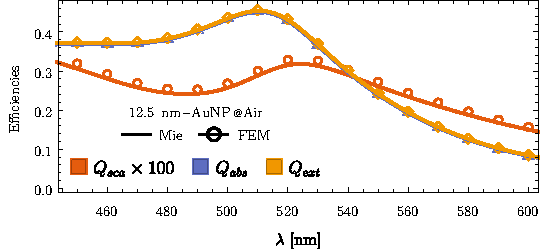
\includegraphics[width = .8\textwidth ]{1-Theory-Figs/Mie-FEM_Air.pdf}\\
%\includegraphics[width = .4\textwidth ]{1-Theory-Figs/Isolated-COMSOL.pdf}%
%\includegraphics[width = .4\textwidth ]{1-Theory-Figs/Isolated-COMSOL.pdf}%
%\caption[Convergence tests: The Meshing]{Resonance wavlength ($\lambda_\text{res}$) of the scattering (orange) and extinction (black) cross sections as functions of the NPs radii when embedded  \ref{sfig:red:1} into air and \ref{sfig:red:2} into water, and as function of the refractive index of the matrix for NP of radius set to  \ref{sfig:red:3} 12.5 nm and \ref{sfig:red:4} 50 nm.}
%\end{figure}




\begin{figure}[h!]\centering
	\def\svgwidth{.8\textwidth} \small
%\includeinkscape{1-Theory-Figs/SistemaBox}
\vspace*{0em}
\caption[Spherical symmetric COMSOL Setup]{A 3D view (left) and the cross section (right) of a spherical symmetric COMSOL setup to calculate the optical response of a single spherical NP embedded into a matrix. The NP (yellow) is located at the center of the matrix (gray), which is covered by a PML layer (blue). The upper layer of the PML is hidden to allow a better view of the setup.}
\label{fig:setup:sphere}
\end{figure}

\begin{figure}[h!]
\def\svgwidth{\textwidth} \small
\hspace*{-1.25em}
\begin{subfigure}{.1\textwidth}\caption{ }\label{fig:Eff:sphere:First:a}\end{subfigure}
\vspace*{12.5em} % Crece la distancia entre as etiquetas
\\
\vspace*{-16.5em} % Crece la distancia entre las etiquetas y el pie de figura
\hspace*{-.75em}%
\begin{subfigure}{.1\textwidth}\caption{ }\label{fig:Eff:sphere:First:b}\end{subfigure}\\
\includeinkscape{FEM/4-Conv}
\vspace*{-1.5em} %Crece la ditancia entre la imagen y el pie de figura
\caption[Scattering, Absorption and Extinction Efficiencies of a 5 nm AuNP$@$Air: Analytical and FEM solutions with no optimizatio]{\textbf{a)} Scattering $Q_\text{sca}$, absorption $Q_\text{abs}$ and extinction $Q_\text{ext}$ efficiencies of a 5 nm AuNP embedded into air calculated by means of the Mie Theory (continuous) and the FEM (disks), and \textbf{b)} their absolute error, as function of the wavelength $\lambda$ of the incident plane wave. The chosen parameters for the FEM calculations were based on the COMSOL Excercises \textbf{CITAR}.}
\label{fig:Eff:sphere:First}
\end{figure}
